% 06.1.7. ESFUERZOS REALES DE LAS PERSONAS Y ROLES 
%----------------------------------------------------------------------------------------

\paragraph{} Se muestran los datos y las gráficas con las horas realizadas por las diferentes personas del equipo en las figuras ~\cref{fig:6171} y ~\cref{fig:6172}. 

\paragraph{} Los roles de los miembros del grupo son los siguientes:
\begin{itemize}
\item Daniel $\Rightarrow$ Director de proyecto
\item Alberto $\Rightarrow$ Verificación y validación
\item Javier $\Rightarrow$ Gestor de configuraciones
\item Héctor $\Rightarrow$ Gestor de calidad
\item Simón $\Rightarrow$ Gestor de desarrollo
\item Alejandro $\Rightarrow$ Gestor de planificación
\end{itemize}

\paragraph{} En la gráfica ~\cref{fig:6171} se ven las diferentes horas invertidas por los integrantes del grupo. Algún aspecto a destacar es que Daniel, como director del proyecto, invirtió el que más horas en el mismo. Además el mes de Marzo, como ya se ha recalcado anteriormente, fue en el que más horas se invirtieron, es decir, ese mes fue el grueso del proyecto. También podemos observar como Javier, al ser el principal encargado de la implementación de la aplicación, tenía una carga de trabajo inicial menor pero después mientras el resto del grupo bajaba el nivel de trabajo él lo subía.

\begin{figure}[h!]
\centering
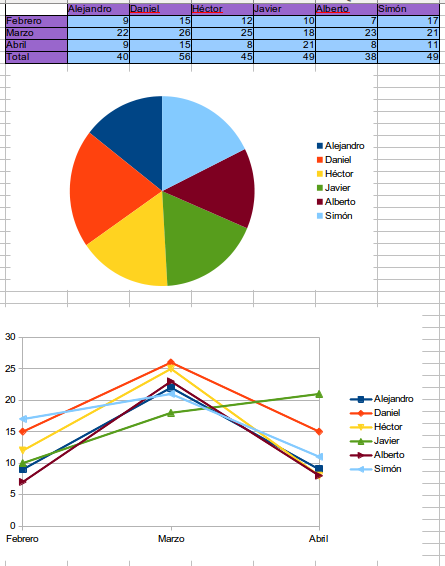
\includegraphics[width=0.95\textwidth]{img/6171}
\caption{Esfuerzos reales por persona primera iteración}
 \label{fig:6171}
\end{figure} 

\paragraph{} Se presentan a continuación los datos para la segunda iteración. De nuevo el director, Daniel, invirtió el que más horas en el proyecto y os demás integrantes del grupo más o menos hicieron las mismas horas de trabajo. Datos que representan una buena organización y reparto de trabajo.

\begin{figure}[h!]
\centering
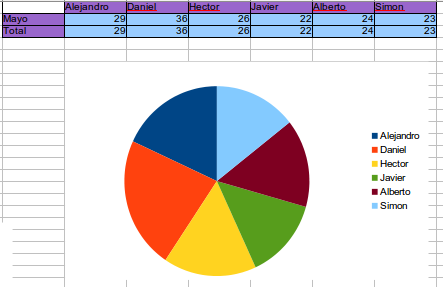
\includegraphics[width=0.85\textwidth]{img/6172}
\caption{Esfuerzos reales por persona primera iteración}
 \label{fig:6172}
\end{figure} 